\documentclass[a4paper,11pt, twocolumn]{article}
%\usepackage[T1]{fontenc} %for å bruke æøå
\usepackage[utf8]{inputenc}
\usepackage[T1]{fontenc}
\usepackage[norsk]{babel}
\usepackage{graphicx} %for å inkludere grafikk
\usepackage{verbatim} %for å inkludere filer med tegn LaTeX ikke liker
\usepackage{mathpazo}
\usepackage{mathtools}
\usepackage{csquotes}
\usepackage{tikz}
\usepackage{listings}
\usepackage{booktabs}
\usepackage{todonotes}
\usepackage[backend=biber]{biblatex}
\usepackage{caption} 
\usepackage{parboxx}
\hyphenpenalty=750
\captionsetup[table]{skip=10pt}

\addbibresource{elastisitet.bib}


\lstset{language=Matlab, commentstyle=\textcolor[rgb]{0.00,0.50,0.00}, keepspaces=true, columns=flexible, basicstyle=\footnotesize, keywordstyle=\color{blue}, showstringspaces=false, inputencoding=ansinew}

\title{Rapport 4 FYS2150\\Elastisitet}

\author{Eivind Brox}
\date{\today}

\begin{document}
\maketitle

\listoftodos

\begin{abstract}

\end{abstract}

\section{Introduksjon}
   
\section{Teori}
Vi ønsket å måle elastisitetsmodulen både ved å se på hvor mye en sylinderstav bøyde seg ved påtrykt kraft, og ved å undersøke hvilken grunnfrekvens staven stabiliserte seg på en stunde etter vi hadde påført en impuls for å sette den i vibrasjon.
\subsection{Nedbøying av stav}
Fra oppgaveteksten for det eksperimentelle arbeidet, \cite{oppgavetekst}, har vi at defleksjonen, $h(m)$, for en bjelke støttet på to punkter, med belastning midt mellom disse punktene er

\begin{equation}
	h(m) = \frac{mgl^3}{48EI}
\end{equation}

Der $mg$ er kraften som virker midt bjelken, $l$ er avstanden mellom punktene bjelken hviler på, $E$ er elastisitetsmodulen og $I$ er andre arealmoment. For en sylinder har vi

\begin{equation}
	I = \frac{\pi d^4}{64}
\end{equation}

Defleksjonen oppfører seg tilnærmet lineært, og finner vi stigningstallet for lineærtilpasningen av målingene våre, $A$, kan vi uttrykke elastisitetsmodulen som  

\begin{equation}
	E = \frac{4l^3g}{3\pi |A|d^4}
	\label{eq:elastisitetsmodulDefleksjon}
\end{equation}

Vi får en usikkerhet på
\begin{equation}
	s_E = E\sqrt{\left(\frac{s_A}{A}\right)^2+\left(\frac{4s_d}{d}\right)^2+\left(\frac{3s_l}{l}\right)^2}	
	\label{eq:feilDefleksjon}
\end{equation}


\subsection{Dynamisk bestemmelse av $E$ ved måling av lydhastighet}
Teorien er også her hentet fra oppgaveteksten \cite{oppgavetekst}. 

Ved å utnytte at elastisitetsmodulen for et material avhenger av hastigheten til lyden i materialet og tettheten til materialet på følgende måte

\begin{equation}
	E = \rho v^2
	\label{eq:dynamiskElastisitet}
\end{equation}

kan vi ved relativt enkle målinger finne et estimat for elastisitetsmodulen. Her er $v$ utbredelseshastigheten for de longitudinale bølgene i materialet vårt og $\rho$ er tettheten til materialet.

Vi utnytter at bølgelengden, $\lambda$, for de longitudinale bølgene for en stav kan beskrives ved 

\begin{equation}
	\lambda = \frac{2L}{n}, \quad n = 1, 3, 5, \dots
\end{equation}

der $L$ er stavens lengde. Vi vet at frekvensen, $f$, er beskrevet ved $f = v/\lambda$, slik at vi får 

\begin{equation}
	v = 2Lf
\end{equation}

ettersom svingningene ved de lengste bølgelengdene er de som dempes saktest. Vi kan dermed uttrykke elastisitetsmodulen som

\begin{equation}
	E = 4\rho(Lf)^2
	\label{eq:dynEl}
\end{equation}

Vi får en usikkerhet på
\begin{equation}
	s_E = E\sqrt{\left(\frac{2s_d}{d}\right)^2+\left(\frac{2s_f}{f}\right)^2+\left(\frac{s_L}{L}\right)^2+\left(\frac{s_m}{M}\right)^2}	
	\label{eq:feilDynamisk}
\end{equation}

\section{Eksperimentelt}
{\bf Utstyr:}

Dimensjoner messingstav og defleksjonsmålinger:
\begin{itemize}
	\item Målebånd, Laufkin 2m Pee Wee Y612CM
	\item Mikrometer, Moore and Wright
	\item Messingstav
	\item Kalibreringslodd: 2kg, 1kg, 100g og 10g
	\item Balansevekt, Ohaus
	\item Stativ med kniver og oppsett for måleur
	\item Skrutrekker
\end{itemize}

Dynamisk måling av elastisitetsmodulen:
\begin{itemize}
	\item Mikrofon, Trust
	\item Høytaler 
	\item Frekvensgenerator \todo[inline]{Finn mer info}
	\item Plasthammer
\end{itemize}

\subsection{Kalibrering av lodd}
Ettersom vi ikke hadde tilgjengelig et referanse lodd på 500g så måtte vi lage en kalibreringskurve for å finne en mer nøyaktig verdi for halvkilosloddet vårt. For å bestemme mer nøyaktige verdier for de grove loddene våre, lagde vi en kalibreringskurve for balansevekten ved bruk av referanselodd. Vi målte hva vekten viste for de forskjellige referanseloddene, etter å først ha stilt den til å vise null utslag når det ikke var lagt på vekt. Vi gjorde deretter en lineær tilpassing som tilnærmet punktene våre på best mulig måte.

\subsection{Defleksjon av messingstav}
For den første metoden av bestemmelse av elastisitetsmodulen benyttet vi et stativ med to kniver som messingstaven vår hvilte på. Vi hengte opp en skål for å legge vekter i midt mellom disse to kivene, og vi plasserte et måleur omtrent i samme posisjon for å måle defleksjonen til messingstaven. Oppsettet er vist i figur \ref{fig:oppsett}.

\begin{figure}[!ht]
\includegraphics[width=0.5\textwidth]{OppsettDefleksjon.png}
\caption{Skjematisk framstilling av oppsettet for måling av defleksjonen av messingstaven \cite{oppgavetekst}.}
\label{fig:oppsett}
\end{figure}

Vi fant også et estimat for diameteren til staven ved en rekke målinger langs staven.

\subsection{Dynamisk måling av elastisitetsmodulen}
For å få messingstaven til å svinge hang vi den opp i det vektene som belastet staven i defleksjonsdelen av oppgaven var hengt opp med, før vi slo på endene av staven med en plasthammer i aksial retning. Dette skaper longitudinale bølger som dempes med tiden. Den bølgen som dempes saktest er den som har størst bølgelengde, og når vi har frekvensen til denne og bølgelengden finner vi hastigheten til lyden i messingen. Dette kan vi sammen med tettheten til staven benytte til estimere elastisitetsmodulen ved ligning \eqref{eq:dynamiskElastisitet}.

Først fant vi den ønskede frekvensen ved å benytte en frekvensgenerator som stod på samtidig som vi hørte lyden fra den vibrerende messingstaven. Vi justerte først på frekvensgeneratorene til lydene hørtes ganske like ut før vi gjorde finjusteringer der vi prøvde å minimere frekvensen til svevelyden vi oppfattet.

Vi gjennomførte også målinger med mikrofon som ble analysert med \textit{fast fourier transform} algoritmen.

\section{Resultater}
Generelle resultater for messingstaven presenteres etter kalibreringen av vektene. Resultatene for de to forskjellige metodene å måle elastisiteten følger deretter, før resultatene sammenlignes.

\subsection{Kalibrering av lodd}

Verdiene i tabell \ref{tab:kalibrering} viser avlest verdi på balansevekten for kalibreringsloddene.

\begin{table}[!ht]
\centering
\caption{Data for kalibrering av balansevekten}
\label{tab:kalibrering}
\begin{tabular}{cc}
	\toprule
	\toprule
	Kalibreringslodd [g] & Balansevekt [g]\\
	\hline
	100 & 99.9\\
	200 & 199.8\\
	1000 & 1000.1\\
	2000 & 2000.2\\
	\toprule
\end{tabular}
\end{table}

Verdiene vi fikk ved å lese av de grove loddene er listet i tabell \ref{tab:kalibrert}, sammen med verdiene vi fant etter å ha brukt kalibreringskurven, funnet ved lineær tilpassing ved bruk av ligninger fra \cite[s. 39]{squires}.

\begin{table}[!ht]
\centering
\caption{Avlest verdi for de grove loddene med balansevekten, sammen med de kalibrerte verdiene.}
\label{tab:kalibrert}
\begin{tabular}{cc}
	\toprule
	\toprule
	Avlest [g] & Kalibrert [g]\\
	\hline
	500.1 & 500.2\\
	1000.2 & 1000.2\\
	2000.6 & 2000.4\\
	\toprule
\end{tabular}
\end{table}

\subsection{Parametre for messingstaven}
Tabell \ref{tab:diameter} viser målingene våre for diameteren til messingstaven og gjennomsnittsverdien og standardfeilen for denne.

\begin{table}[!ht]
\centering
\caption{Forskjellige målinger for messingstavens diameter, gjennomsnittsverdien og standardfeilen for gjennomsnittsverdien.}
\label{tab:diameter}
\begin{tabular}{ccc}
	\toprule
	\toprule
	 & D[mm]&\\
	\hline
	15.99 & 15.99 & 16.01\\
	16.00 & 15.99 & 15.99\\
	16.00 & 16.00 & 15.99\\
	\hline
	mean & 15.996 &\\
	$\sigma_m$ & 0.00081&\\
	\toprule
\end{tabular}
\end{table}

Lengden av messingstaven målte vi med målebåndet vårt til å være 144,4cm. Vi anslo at usikkerhet var på 0.2cm ettersom det var litt slark i festeanordningen på enden av målebåndet. Vi har dermed 

\begin{equation}
L=144.4\pm0.2\text{cm} 
\end{equation}

Med balansevekten målte vi massen til messingstaven til å være 2447.9g.  Dette gjorde vi ved først å skru av den horisontale måleplaten, legge denne på balansevekten, og stille inn offset-skruen slik at vekten viste null. Vi skrudde deretter på måleplaten og veide staven. Hvis vi ekstrapolerer for kalibreringskurven vår får vi 2447.6g. Vi anslo usikkerheten til å ligge innenfor 0.5g slik at vi får

\begin{equation}
	M = 2447.6\pm0.5\text{g}
\end{equation} 

Usikkerheten for mikrometeret er angitt til å være 0.02mm, som er mye større enn standardfeilen funnet for målingene vi gjorde. Vi velger derfor å benytte 0.02mm som usikkerhet, slik at

\begin{equation}
	D = 16.00\pm0.02\text{mm}
\end{equation}

\subsection{Defleksjon av messingstav}
Vi målte defleksjonen til messingstaven ved å belaste den med alle kombinasjonene av de tre loddene vi hadde tilgjengelig. Resultatene er presentert i tabell \ref{tab:defleksjon}.
\begin{table}[!ht]
\centering
\caption{Målinger for defleksjonen av messingstaven.}
\label{tab:defleksjon}
\begin{tabular}{cc}
	\toprule
	\toprule
	Lodd [g] & Verdi måleur [mm]\\
	\hline
	uten lodd & 9.78\\
	500.1 & 9.06\\
	1000.2 & 8.33\\
	1500.3 & 7.60\\
	2000.4 & 6.88\\
	2500.5 & 6.15\\
	3000.6 & 5.40\\
	3500.7 & 4.67\\
	\toprule
\end{tabular}
\end{table}

Det interessante her er stigningstallet for den lineære tilpassingen av dataene. Vi finner igjen denne ved å bruke ligningene fra \cite[s. 39]{squires}. Vi får dermed et stigningstall på $A = -0.00146$mm/g, med en feil på $s_A=2.78\cdot10^{-6}$mm/g. Vi oppgir dermed stigningstallet som

\begin{equation}
	A = -(1.459\pm0.003)\cdot10^{-3}\text{
m/kg}
\end{equation}

Lengden mellom de to knivene som messingstangen hvilte på (B og C i figur \ref{fig:oppsett}) fant vi til å være 

\begin{equation}
	l = 1.339\pm0.002\text{m}
\end{equation} 
der usikkerheten er anslått på samme måte som målingen av lengden for hele staven.

Ved bruk av ligning \eqref{eq:elastisitetsmodulDefleksjon} estimerer vi dermed elastisitetsmodulen til å være

\begin{equation}
	E = \frac{4\cdot(1.339\text{m})^3\cdot9.82\text{m/s}^2}{3\pi\cdot 1.459\cdot (0.016\text{m})^2} \approx 104.57\text{GPa}
\end{equation}

Usikkerheten finner vi ved ligning \eqref{eq:feilDefleksjon}

\begin{align}
	s_E &= E\sqrt{\left(\frac{0.003}{1.459}\right)^2+\left(\frac{4\cdot0.02}{16.0}\right)^2+\left(\frac{3\cdot 2}{1339}\right)^2}\\
	&= 561\text{MPa}\\
	&\implies \underline{E = 104.6\pm0.6\text{GPa}}
\end{align}


\subsection{Dynamisk måling}
For metoden med svevelyd kom vi fram til en frekvens på 1213Hz, der vi anslo at usikkerheten i forhold til hvor godt vi hørte lyden, og hvor nøye vi stilte inn frekvensgeneratoren burde ligge innenfor 0.5Hz. 

For fourieranalysen fant vi en frekvens på 1213.2Hz. Målingen vi benyttet varte i 10 sekunder, som gir en frekvensoppløsning på 0.1Hz \cite{vistnes4}. Usikkerheten er nok litt større ettersom signalet er tidsvarierende og hammerslaget fant sted etter at målingene var påbegynt. Figur \ref{fig:frekvensspekter} viser frekvensspekteret vi fant for lyden vi tok opp.

\begin{figure}[!ht]
	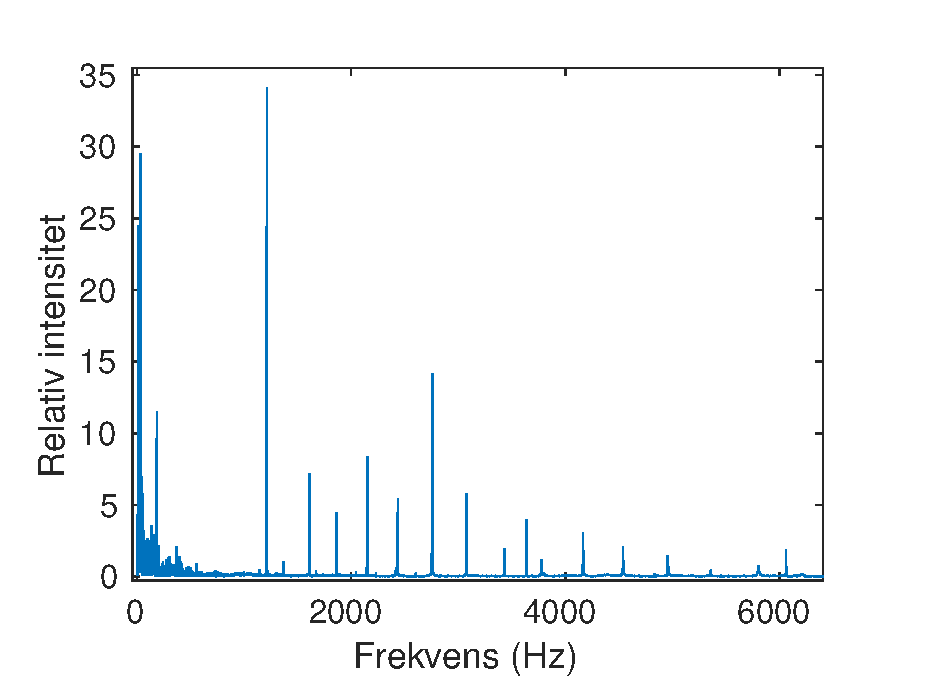
\includegraphics[width = 0.5\textwidth]{matlab/frekvensspekter.eps}
	\caption{Frekvensspekter fra 10 sekunders måling av lyden fra den vibrerende messingstaven.}
	\label{fig:frekvensspekter}
\end{figure}

Når vi vet dette kan vi bytte ut tettheten i ligning \eqref{eq:dynEl} med formelen for tettheten til en sylinder, og få

\begin{align}
	E &= \frac{16Lf^2M}{\pi d^2}\\
	&=\frac{16\cdot 1.444\text{m}\cdot(1213.2Hz)^2\cdot2.4476\text{kg}}{\pi (0.016\text{m})^2}\\
	&= 103.49\text{GPa}
\end{align}

Usikkerheten finner vi til å være $s_E = 0.133$GPa ved å bruke ligning \ref{eq:feilDynamisk}. Dette gir oss en elastisitetsmodul på

\begin{equation}
	E = 103.5\pm1\text{GPa}
\end{equation}

\section{Diskusjon}


\section{Konklusjon}

\printbibliography
\clearpage
\onecolumn
\appendix


%\section{Matlab-script}

\end{document}
